\section{Design of UPRESSO}
\label{sec:UPRESSO}
In this section, we provide designs of UPRESSO, a secure and privacy-preserving SSO system.
First, we present how to achieve the trapdoor user identification and transformed receiver designation. Then, we describe the detailed protocol for providing the SSO service. Finally, we discuss the compatibility of UPRESSO with OIDC.

\subsection{Features}
\label{subsec:overview}
The three functions $F_{PID_{RP}}$, $F_{PID_U}$ and $F_{Account}$  are essential for the trapdoor user identification and  transformed receiver designation.
In UPRESSO, these functions are constructed based on discrete logarithm cryptography with the public parameters $p$, $q$, $g$ and $N$,
 where  $p$ is a large prime defines the finite field $GF(p)$, $N$ is the length of $q$, $q$ ($2^{N-1} < q < 2^N$) is a prime divisor of ($p-1$), and $g$ is a generator of order $q$.
%the prime number $q$  is the order of a multiplicative subgroup of $GF(p)$, which is generated with the generator $g$ by $\{g\ mod\ p, g^2\ mod\ p, ..., g^{q-1}\ mod\ p, 1=g^q\ mod\ p\}$.

In UPRESSO, IdP assigns a  random number as  $ID_U$ ($0 < ID_U <q $)  at the user's registration, and chooses a random number $r$ ($1 < r < q$) to generate $ID_{RP}$ at the RP’s initial registration. The $r$ must be different from the ones chosen before, and $ID_{RP}$ is generated using Equation~\ref{equ:IDRP}.
 
\begin{equation}
    ID_{RP} = g^{r} mod \ p
   \label{equ:IDRP}
\end{equation}


For each login, the RP chooses a random number $n_{RP}$ ($1 < n_{RP}<q $), the user chooses a random number $n_{U}$ ($1 < n_{U}<q $). Then, the RP and user cooperatively  generate $PID_{RP}$ using the function $F_{PID_{RP}}$ as Equation~\ref{equ:PIDRP}. The function $F_{PID_{RP}}$ satisfies the requirements described in Section~\ref{subsec:challenges}. That is, the function $F_{PID_{RP}}$ is invoked to generate $PID_{RP}$ for each login, while IdP  fails to derive $ID_{RP}$ from $PID_{RP}$ and cannot find the relation among ${PID_{RP}}$s for a same RP, which is ensured by the discrete logarithm cryptography.
Moreover, $n_{U}$ and $n_{RP}$  serves as the nonce which ensures that the $PID_{RP}$ (also identity proof) is exactly constructed for this login, and
the cooperation between the user and RP prevents the malicious user and RP from controlling the  $PID_{RP}$. For example, the malicious user fails to make a correct RP accept a $PID_{RP}$ used in another login, while the collusive RPs fail to use a same or correlated $PID_{RP}$s for different logins.


 \begin{equation}
    PID_{RP} = {ID_{RP}}^{n_{u}* n_{RP}} mod \ p
   \label{equ:PIDRP}
   \end{equation}

For the user $ID_U$ to login at an RP with a privacy-preserving identifer $PID_{RP}$, IdP calculates the user's privacy-preserving identifer $PID_U$ using the function  $F_{PID_{U}}$ as Equation~\ref{equ:PIDU}. The function $F_{PID_{U}}$ satisfies the requirements described in Section~\ref{subsec:challenges}.
Combining Equation~\ref{equ:IDRP}, ~\ref{equ:PIDRP} and~\ref{equ:PIDU}, we get that  $PID_U$ equals to $g^{r*n_U*n_{RP}*ID_U}\ mod \ p$.
The discrete logarithm cryptography ensures that the RPs fail to derive $ID_U$ from $PID_U$,
nor link a user's $PID_U$s at different RPs who can never  know $r$ and $ID_U$. %have different $ID_{RP}$. %discrete logarithm of $ID_{RP}$ modulo $ID_{RP}^'$


\begin{equation}
 PID_U = {PID_{RP}}^{ID_U} \ mod \ p
 \label{equ:PIDU}
\end{equation}

Finally, the RP derives $Account$ for the user with the function $F_{Account}$ as Equation~\ref{equ:Account}. Here, the value $(n_U*n_{RP})^{-1} mod \ q$ is the trapdoor $t$. As $q$ is a prime number, $1< n_U < q$ and $1< n_{RP} < q$, therefore $q$ is coprime to $n_U*n_{RP}$, and the $t$ that satisfies $t*(n_U*n_{RP}) = 1\ mod \ q$ always exists. The function $F_{Account}$ satisfies the requirements described in Section~\ref{subsec:challenges}.  As shown in Equation~\ref{equ:AccountNotChanged},  for a user's multiple logins at an RP, $F_{Account}$ outputs an unchanged $Acount$  which equals to ${{ID_{RP}}^{ID_U}} mod \ p$.
Same as the analysis of $PID_U$, the collusive RPs fail to derive $ID_U$ from $Account$ nor link a user's $Account$s due to the different and unknown $r$s.

 \begin{equation}
   Account = {PID_U}^{(n_U*n_{RP})^{-1} mod \ q} mod \ p
   \label{equ:Account}
   \end{equation}

The \textbf{trapdoor user identification} is supported with these three functions.
For a user's multiple logins, each PR obtains the different $PID_U$s and the corresponding $t$s , then derives the unchanged $Account$  as shown in Equation~\ref{equ:AccountNotChanged}.
The function $F_{PID_{RP}}$ prevents the curious IdP from linking the $PID_{RP}$s of different logins at an RP, and therefore avoids  the  IdP-based access tracing.
The functions $F_{PID_{U}}$ and $F_{Account}$ prevents the collusive RPs from linking a user's $PID_U$s and $Account$s at different RPs, and therefore avoids the RP-based identity linkage.
 \begin{multline}\label{equ:AccountNotChanged}
   Account =  {PID_{U}}^{t} mod \ p  \\
   = {({PID_{RP}}^{ID_U})}^{{(n_U*n_{RP})^{-1} mod \ q}} mod \ p \\
   = {ID_{RP}} ^ {ID_U * n_U * n_{RP} *t\ mod\ q} = {ID_{RP}}^{ID_U} mod \ p
 \end{multline}

The \textbf{transformed receiver designation} is also supported with the efficient functions $F_{PID_{RP}}$ and $F_{PID_U}$, together with  a user-centric verification.
The $F_{PID_{RP}}$ ensures that the user and RP cooperatively generate a fresh $PID_{RP}$  for a user's login,
 while $F_{PID_U}$ ensures that the IdP generates the exact $PID_U$ for the $ID_U$ who logins at $PID_{RP}$.
The IdP will bind $PID_{U}$ with $PID_{RP}$ in the identity proof, which designates this identity proof to $PID_{RP}$.
In the user-centric verification,  the user checks that $PID_{RP}$ is global unique and exactly generated for the RP $ID_{RP}$,
 and then sends the identity proof  only  to this RP. Therefore, the $PID_{RP}$ is designated to $ID_{RP}$.
Finally, the transformed receiver designation is provided through the two-step designations.


\begin{table}[tb]
    \caption{The notations used in UPRESSO.}
    \centering
    \begin{tabular}{|c|c|c|}
    \hline
    {Notation} & {Definition} & {Attribute} \\
    \hline
    {$p$} & {A large prime.} & {Long-term} \\
    \hline
    {$q$} & {A large prime.} & {Long-term} \\
    \hline
    {$N$} & {Length of $q$. } & {Long-term} \\
    \hline
    {$g$} & {A generator of order $q$. } & {Long-term} \\
   % \hline
    %{$SK_{ID}$, $PK$} & {The private/public key to sign/verify identity proof.} & {System-unique} \\
    \hline
    {$ID_U$} & {User's unique identifier.} & {Long-term} \\
    \hline
    {$PID_U$} & {User's privacy-preserving identifier.} & {One-time}\\
    \hline
    {$Account$} & {User's identifier at an RP.} & {Long-term} \\
    \hline
    {$ID_{RP}$} & {RP's original identifier.} & {Long-term} \\
    \hline
    {$PID_{RP}$} & {RP's privacy-preserving identifier.} & {One-time} \\
    \hline
    {$n_U$} & {User-generated random nonce for $PID_{RP}$.} & {One-time} \\
    \hline
    {$n_{RP}$} & {RP-generated random nonce for $PID_{RP}$.} & {One-time} \\
    \hline
    {$Y_{RP}$} & {Public value for $n_{RP}$, $(ID_{RP})^{n_{RP}} \ mod\ p$.} & {One-time} \\
    \hline
    {$t$} & {A trapdoor, $t=(n_U*n_{RP})^{-1} mod \ q$.} & {One-time} \\
    \hline
    {$Cert_{RP}$} & {An RP certificate. } & {Long-term} \\
    \hline
    {$SK$, $PK$} & {The private/public key of IdP. } & {Long-term} \\
     \hline
    \end{tabular}
    \label{tbl:notations}
\end{table}

\subsection{The implementations of UPRESSO}
\label{implementations}
UPRESSO contains four sub-protocols, i.e., system initialization, RP initial registration, user registration and SSO login.
The system initialization is invoked by the IdP to initialize the SSO system and only needs to be invoked once for each SSO system.
The RP initial registration is invoked by each RP to obtain the necessary parameters (a unique identifier $ID_{RP}$ and an RP certificate $Cert_{RP}$) from the IdP and only needs to be invoked once for each RP.
The user registration is only invoked once by each user to create a unique user identifier $ID_U$ and the corresponding credential.
While, the SSO login is invoked once a user wants to log in an RP, and therefore will be invoked frequently.
The process for user registration is the same as the one in the typical SSO systems,
therefore, we focus on the processes in  system initialization, RP initial registration and SSO login.
For clarity, we list the used notations  in Table~\ref{tbl:notations}.

\vspace{1mm}\noindent \textbf{System initialization.} The IdP chooses $N$, generates a large prime $p$, a prime $q$ of $N$ bits, and a generator $g$ of order $q$ as  the parameters for the discrete logarithm cryptography~\cite{gallagher2013digital}, and generates one asymmetric key pair ($SK$ denotes the private key and $PK$ is the public key) for the generation of the identity proof and $Cert_{RP}$.
The IdP keeps $SK$ secretly, and provides $p$, $q$, $g$, $N$ with $PK$ as the public parameters.
The values of $p$, $q$, $g$ and $N$ remain the same during the full lifecycle of an SSO system.
While, the asymmetric key pair ($SK$, $PK$) will be updated when necessary. For example, when $SK$ is leaked, IdP must update ($SK$,$PK$).

\vspace{1mm}\noindent\textbf{RP initial registration.}
The RP initial registration is invoked only once by an RP, to apply $ID_{RP}$ and $Cert_{RP}$ from IdP.
The detailed processes are as follows:
\begin{enumerate}
\item RP sends a request $Req_{Cert_{RP}}$ to the IdP. The $Req_{Cert_{RP}}$ contains the RP's distinguished name $Name_{RP}$ (e.g., DNS name) and the endpoint for receiving the identity proof.
\item IdP calculates a unique $ID_{RP}$ using Equation~\ref{equ:IDRP},  generates the signature $Sig_{SK}$ of [$ID_{RP}, Name_{RP}$] with $SK$, and returns [$ID_{RP}, Name_{RP}, Sig_{SK}$] as $Cert_{RP}$.
\item The RP  verifies $Cert_{RP}$ using $PK$,  and stores $ID_{RP}$ with the valid $Cert_{RP}$ for the further use.
\end{enumerate}

\vspace{1mm}\noindent\textbf{SSO login.}
Once a user attempts to log in at an RP, the SSO login is invoked. We use the OIDC implicit protocol flow as an example, to demonstrate  how to integrate the three functions $F_{PID_U}$, $F_{PID_{RP}}$ and $F_{Account}$ into the typical SSO systems.
As shown in Figure~\ref{fig:UPRESSO}, the SSO login sub-protocol contains four phases, RP identifier transforming, RP identifier refreshing, $PID_U$ generation and $Account$ calculation.
In the RP identifier transforming, the user and RP negotiate $PID_{RP}$ based on Diffie-Hellman key exchange~\cite{DiffieH76}, where $PID_{RP}$ is calculated as in Equation~\ref{equ:PIDRP}.
In the RP identifier refreshing, the user registerers the unique  $PID_{RP}$ at IdP.
In the $PID_U$ generation, IdP calculates $PID_U$ with $ID_U$ and $PID_{RP}$ as in Equation~\ref{equ:PIDU}.
And in the $Account$ calculation, the RP derives the unchanged $Account$ as in Equation~\ref{equ:Account}.

\subsection{Overall protocol flow overview}
\label{sebsec:loginprocess}
In UPRESSO, the SSO login sub-protocol provides the secure SSO service and prevents both the IdP-based access tracing and RP-based identity linkage.
The protocol, shown in Figure~\ref{fig:process},  prevents the curious IdP from obtaining the RP's identifying information during the interchanges,
  and avoids the adversary to break the security and user's privacy.
Here we introduce the detailed processes for each step in Figure~\ref{fig:process}.

\begin{figure*}
  \centering
  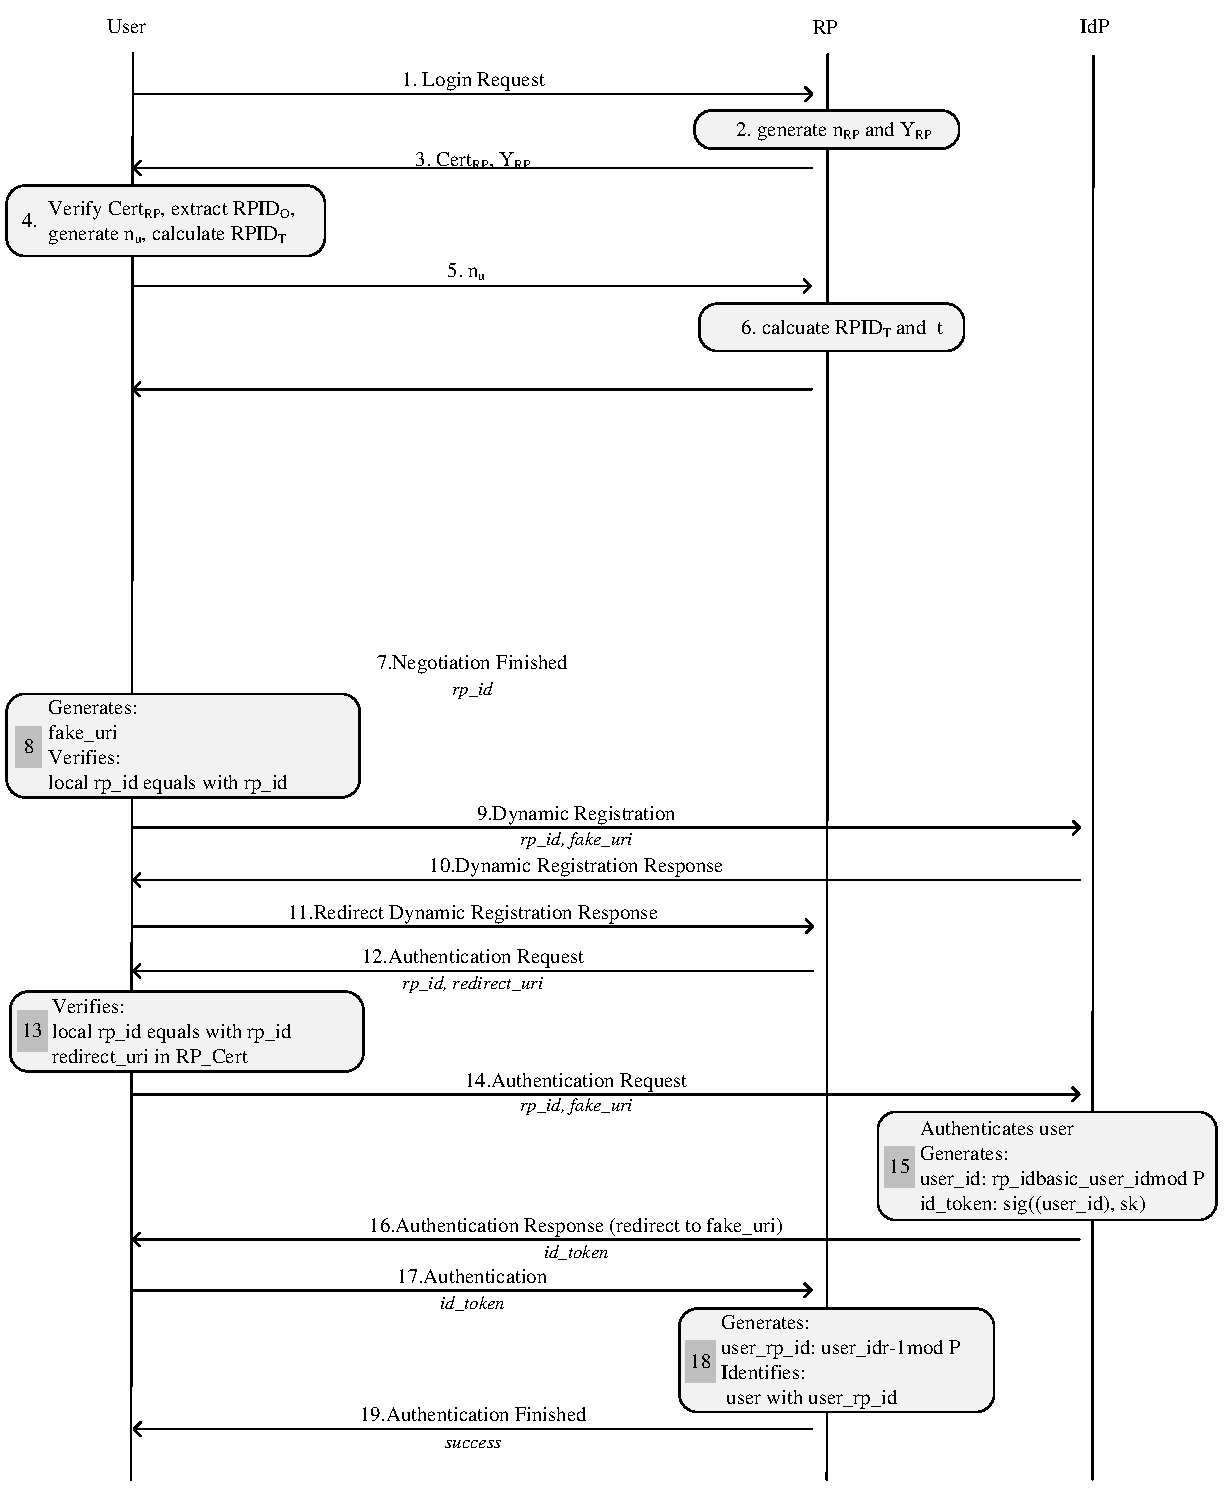
\includegraphics[width=0.85\linewidth]{fig/process.pdf}
  \caption{Process for each user login.}
  \label{fig:process}
\end{figure*}

\vspace{1mm}\noindent\textbf{RP identifier transforming.}
In this phase, the user and RP cooperative to generate $PID_{RP}$ as follows:
\begin{itemize}
  \item The user sends a login request to trigger the negotiation of $PID_{RP}$ (Step 1).
  \item The RP chooses a random $n_{RP}$ ($1 < n_{RP} <q$), calculates $Y_{RP}={ID_{RP}}^{n_{RP}} mod \ p$ (Step 2.1.1); and sends $Cert_{RP}$ with $Y_{RP}$ to the user (Step 2.1.2).
  \item The user checks the $Cert_{RP}$, extracts $ID_{RP}$ from the valid $Cert_{RP}$, chooses a random $n_U$ ($1 < n_U <q$) to calculate $PID_{RP}={Y_{RP}}^{n_{u}} mod \ p$ (Step 2.1.3); and sends $n_U$ with $PID_{RP}$ to the RP (Step 2.1.4).
  \item The RP calculates $PID_{RP}$ with $n_U$ and $Y_{RP}$, checks its consistency with the received one, derives the trapdoor $t={(n_U*n_{RP})}^{-1} \ mod \ q$ (Step 2.1.5); and sends the calculated $PID_{RP}$ to the user (Step 2.1.6).
  \item The user checks the consistency of the received $PID_{RP}$ with the stored one.
\end{itemize}
During the process, the user will halt the login, if  the $Cert_{RP}$ is invalid or the received $PID_{RP}$ is different from the stored one. The RP also halts the process if the $PID_{RP}$ sent by the user is inconsistent with the calculated one.

\vspace{1mm}\noindent\textbf{RP identifier refreshing.}
The user registers $PID_{RP}$ at the IdP as follows.
\begin{itemize}
  \item The user generates an one-time endpoint to hide the RP's endpoint from IdP (Step 2.2.1), and sends the registering request [$Reg$, $PID_{RP}$, one-time endpoint] to the IdP (Step 2.2.2).
  \item The IdP checks $PID_{RP}$, and constructs the response [$RegRes$, $RegMes$, $Sig_{Reg}$] (Step 2.2.3). The $RegRes$ is registration result, and is set as $OK$ only when $PID_{RP}$ is never used before and is of order $q$ module $p$. The $RegMes$ is the same as the dynamic registration response, and contains $PID_{RP}$, the issuing time and valid time. The $Sig_{Reg}$ is the signature for $RegRes$ and $RegMes$ generated by the IdP with $SK$.
  \item The user accepts $RegRes$ directly due to the secure connection with IdP, and forwards the registration result to the RP (Step 2.2.4).
  \item The IdP checks $Sig_{SK}$ and $RegMes$, and accepts $RegRes$ only when $Sig_{Reg}$ is valid, $PID_{RP}$ is the same as the negotiated one, and $RegMes$ is not expired.
\end{itemize}
If $RegRes$ is $OK$, the RP identifier refreshing completes. Otherwise, the user and RP will renegotiate the $PID_{RP}$.

\vspace{1mm}\noindent\textbf{$\mathbf{PID_U}$ generation.}
In this phase, the RP continues the process of the user's login and obtains the $PID_U$ generated by the IdP. The processes are as follows.
\begin{itemize}
  \item The RP uses $PID_{RP}$ and the endpoint to construct an identity proof request, which is the same as the one in  OIDC. (Step 2.3).
  \item The user checks the consistency of the received $PID_{RP}$  with the negotiated one (Step 2.4); replaces the endpoint with the one-time endpoint generated in Step 2.2.1, and sends the modified identity proof request to the IdP (Step 2.5).
  \item The IdP authenticates the user if she hasn't been authenticated (Step 3); checks whether $PID_{RP}$ and the one-time endpoint have been registered,
   calculates $PID_U$ using Equation~\ref{equ:PIDU},  constructs the identity proof [$PID_{RP}$, $PID_U$, $ValTime$, $Attr$,$Sig_{IdProof}$] where $ValTime$ is the valid period, $Attr$ contains the  attributes that the user agrees to provide to the RP, $Sig_{IdProof}$ is the signature of the identity proof generated by IdP with $SK$ (Step 4). Then, the IdP sends the identity proof with the one-time endpoint to the user (Step 5.1).
  \item The user finds  the  endpoint corresponding to the one-time endpoint (Step 5.2),
   and forwards the identity proof to the RP through this endpoint (Step 5.3).
\end{itemize}
The user halts the process if the $PID_{RP}$ in the identity proof request is inconsistent with  the negotiated one.
The IdP rejects the identity proof request, if the $PID_{RP}$ and the one-time endpoint have not been registered.


\vspace{1mm}\noindent\textbf{$\mathbf{Account}$ calculation.}
Finally, RP derives the user's  $Account$ and completes the user's login as follows. The RP performs the checks on the identity proof, including the valid time, correctness of $Sig_{IdProof}$, and   the consistency between $PID_{RP}$ and the  negotiated one. If all the checks pass, the RP extracts $PID_U$, and calculates $Accout$ according to Equation~\ref{equ:Account} (Step 6); and sends the $Success$ as the login result to the user (Step 7). If any check fails, the RP returns the $Fail$ to the user.


\subsection{Compatibility with OIDC}
\label{subsec:compatible}
UPRESSO could be integrated in the traditional SSO systems, to  prevent the IdP-based access tracing and RP-based identity linkage.
The integration doesn't degrade the security and only requires minimal modification.
Here, we use the implicit protocol flow of OIDC as an example to demonstrate the compatibility of UPRESSO with the traditional SSO systems.
The further analysis, such as integration with the authorization code flow of OIDC,  is provided in Section~\ref{sec:discussion}.


\vspace{1mm}\noindent \textbf{Consistency with OIDC.}
As shown in Figure~\ref{fig:UPRESSO}, the architecture of UPRESSO is the same as the one in OIDC. UPRESSO does not introduce any new entity, but only integrates the three function $F_{PID_U}$, $F_{PID_{RP}}$ and $F_{Account}$ into the processes at the IdP, RP, and user.

The formats of the  identity proof and corresponding request, and the verification of the identity proof,  are almost same in OIDC and UPRESSO.
The only difference is that $ID_{RP}$ and endpoint are replaced with the privacy-preserving versions, i.e., $PID_{RP}$ and one-time endpoint, in UPRESSO.
As $PID_{RP}$ is also unique and corresponds exactly to $ID_{RP}$, and one-time endpoint corresponds to the RP's endpoint correctly,
 the binding, integrity and confidentiality of identity proof will also be ensured in UPRESSO, and there is no degradation on the security of OIDC.

\vspace{1mm}\noindent \textbf{Minimal modification to OIDC.}
UPRESSO only requires small modification on OIDC to integrate $F_{PID_U}$, $F_{PID_{RP}}$ and $F_{Account}$.
For $F_{PID_U}$ and $F_{Account}$ , we directly use them to replace original functions for $PPID$ at the IdP and the $Account$ at the RP.
For $F_{PID_{RP}}$, we inject a negotiation process and a dynamic registration for each SSO login,
 where the negotiation process between the user and RP generates a $PID_{RP}$,
  while the dynamic registration is used to check the uniqueness of $PID_{RP}$.
In UPRESSO, the dynamic registration is slightly modified as follows: an RP identifer ($PID_{RP}$)  is added in the request, and a signature ($Sig_{Res}$)  is included in the response for its verification at the RP.





